\documentclass[conference]{IEEEtran}
\IEEEoverridecommandlockouts
% The preceding line is only needed to identify funding in the first footnote. If that is unneeded, please comment it out.
%Template version as of 6/27/2024

\usepackage{cite}
\usepackage{float}
\usepackage{siunitx}
\usepackage{hyperref}
\hypersetup{
colorlinks=true,
linkcolor=blue,
filecolor=magenta,      
urlcolor=blue,
citecolor=blue,
}
\usepackage{amsmath,amssymb,amsfonts}
\usepackage{algorithmic}
\usepackage{graphicx}
\usepackage{textcomp}
\usepackage{xcolor}
\def\BibTeX{{\rm B\kern-.05em{\sc i\kern-.025em b}\kern-.08em
    T\kern-.1667em\lower.7ex\hbox{E}\kern-.125emX}}
\begin{document}

\title{Two-Dimensional Materials in Electronics\\
}

\author{\IEEEauthorblockN{Michael Brodskiy}
\IEEEauthorblockA{\textit{College of Engineering} \\
\textit{Northeastern University}\\
Boston, MA\\
\href{mailto:Brodskiy.M@Northeastern.edu}{Brodskiy.M@Northeastern.edu}}
\and
\IEEEauthorblockN{Thomas Czartoryski}
\IEEEauthorblockA{\textit{Khoury College of Computer Science} \\
\textit{Northeastern University}\\
Boston, MA\\
\href{mailto:Czartoryski.T@Northeastern.edu}{Czartoryski.T@Northeastern.edu}}
\and
\IEEEauthorblockN{Oluwalaanu Adeboye}
\IEEEauthorblockA{\textit{College of Engineering} \\
\textit{Northeastern University}\\
Boston, MA\\
\href{mailto:Adeboye.O@Northeastern.edu}{Adeboye.O@Northeastern.edu}}
\and
\IEEEauthorblockN{Daniela Salazar}
\IEEEauthorblockA{\textit{College of Engineering} \\
\textit{Northeastern University}\\
Boston, MA\\
\href{mailto:Salazar.Dani@Northeastern.edu}{Salazar.Dani@Northeastern.edu}}
\and
\IEEEauthorblockN{John Bergin}
\IEEEauthorblockA{\textit{College of Engineering} \\
\textit{Northeastern University}\\
Boston, MA\\
\href{mailto:Bergin.J@Northeastern.edu}{Bergin.J@Northeastern.edu}}
\and
\IEEEauthorblockN{Owen Chiu}
\IEEEauthorblockA{\textit{College of Engineering} \\
\textit{Northeastern University}\\
Boston, MA\\
\href{mailto:Chiu.O@Northeastern.edu}{Chiu.O@Northeastern.edu}}
}

\maketitle

\begin{abstract}
  The following is a meta-analysis which delves into the field of two-dimensional (2D) materials within the realm of electronics. Key materials under scrutiny include graphene, molybdenum disulfide (MoS$_2$), and hexagonal boron nitride (hBN). This document and the research herein will then be used to generate an accompanying presentation.
\end{abstract}

\begin{IEEEkeywords}
  \underline{meta-analysis}, \underline{two-dimensional materials}, \underline{electronics}, \underline{graphene}, \underline{hBN}, \underline{MoS$_2$}
\end{IEEEkeywords}

\section{Introduction}

Two-dimensional (2D) materials are a mere one or two atoms thick but have a tremendous impact on the electronics industry. One of the more interesting aspects of these materials is that most allow for the transfer of electrons within them and, thus, are conductive. This holds tremendous promise within the semiconductor industry, which has primarily been a silicon-dominated industry. Though silicon has been revolutionary for the electronics industry, this next generation of semiconductors may stray from this silicon-based norm. Traditional semiconductors experience a host of imperfections as scaling continues to increase, including leakage currents, thermal dissipation issues, and short-channel effects \cite{intro}. Unlike their bulk material semiconductor counterparts, 2D materials have exceptional electrostatic control, which is a result of their thin atomic thickness. This has allowed for the construction of ultra-scaled field effect transistors (FETs) that are much more power-efficient than a silicon FET. 

Discussed in this paper are a host of promising 2D materials pertaining to a wide range of applications. Graphene has a carrier mobility of $200,000 [\si{\centi\meter\squared\per\volt\per\second}]$ \cite{mb3}, which is significantly higher than that of silicon. This indicates the potential within a host of devices, including ultra-fast transistors, RF devices, and ultra-sensitive sensors with the capability to outperform the current market of devices due to its high carrier mobility. Hexagonal boron nitride (hBN) is another material that holds promise, specifically in deep-ultraviolet applications, due to its bandgap falling within that range. Other materials, such as silicene and MoS$_2$, may have uses within the ultra-fast transistor market and optoelectronics market, respectively. Silicene’s high carrier mobility makes it a suitable candidate like graphene, but it is much simpler to synthesize. MoS$_2$ has a bandgap of $1.8[\si{eV}]$ \cite{oc3}, thus making it viable for optoelectronics, including photodetectors and LEDs. 

Another important attribute of 2D materials is the capability to create complex heterostructures, which are simply vertical stacks of different 2D materials. This allows for a customizable component, which facilitates device architectures such as tunneling FETs \cite{intro}. 

This creates various ways to manipulate these materials, such that they can be stacked, bent, twisted, etc., to create different effects. This attribute may allow for customizable electronic circuits, p-n junction uses, and computer memory applications. The main drawback for these heterostructures is the difficulty in replication and fabrication. There is a tremendous margin of error within these structures, but with upcoming hope for strides in fabrication processes, it is expected to stimulate the integration of 2D materials within heterostructures for devices \cite{jb3, oc1}.

One of the detrimental challenges of 2D materials is the difficulty of synthesis, particularly in a consistent and scalable manner. This has limited the functionality and implementations of these materials, but the future holds promise in unlocking the full capability of these materials. A perpetuating challenge is achieving large-scale, uniform growth, as current processes often result in a surplus of defects, rendering the material unusable. Chemical vapor deposition is a process that is often used, but its scalability has been limited per current literature. This is due to its ability to produce the size required for a wafer, but these wafers introduce deleterious defects, such as grain boundaries that degrade the electronic performance \cite{intro}. The lack of control of layer thickness is another challenge, as monolayer films require tuning to control a host of parameters (temperature, pressure, etc.), while multilayer or heterostructures require even more. This is primarily due to material instability, which requires perfection in regard to the fabrication environment. Though synthesis remains one of the largest challenges in 2D materials, the promise these materials hold is encouraging. With breakthroughs in the synthesizing process, such as with hBN in monolayer and multilayer applications \cite{jb3, oc1}, the future appears bright for these materials.

\section{Graphene — Michael Brodskiy}

\subsection{Material Structure}

The atomic structure of graphene consists of a single layer of carbon atoms in the formation of a two-dimensional hexagonal lattice (shown in Figure \ref{fig:1}). This structure makes graphene one of the most promising materials within the realm of electronics, as it allows for exceptional electrical, mechanical, and thermal properties \cite{mb1}. These properties contribute to graphene's high carrier mobility and physical strength, which has led to its integration into transistors, and, subsequently, touch screen and energy storage devices \cite{mb2}. The structure can be more thoroughly analyzed by breaking down the scope into three categories:

\begin{figure}[h]
  \centering
  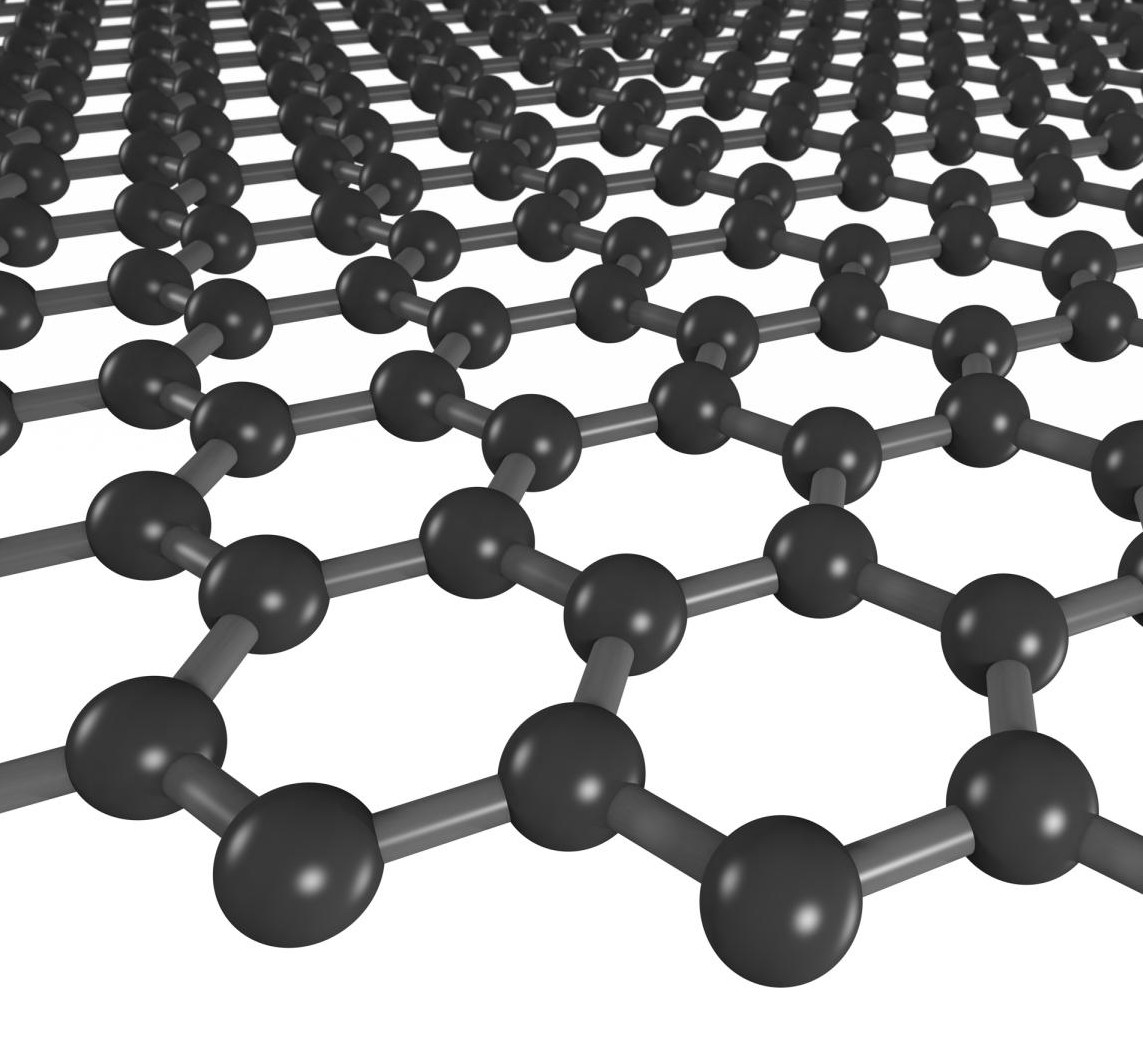
\includegraphics[width=.4\textwidth]{Figures/Graphene}
  \caption{Structure of Graphene}
  \label{fig:1}
\end{figure}

\begin{enumerate}

  \item Atomic Arrangement — Each carbon atom in graphene is bonded to three other carbon atoms at $120^{\circ}$ angles, forming a planar structure. This arrangement allows for a particularly stable formation while ensuring that the fourth valence electron of each carbon atom remains de-localized. The presence of these $\pi$-electrons leads to high electrical conductivity.

  \item Band Structure — The band structure of graphene is characterized by a zero bandgap semi-metal property, effectively making it a unique material for electronic applications. The conduction and valence bands meet at the Dirac points, where electrons behave like massless Dirac fermions, enabling high mobility and speed in electronic devices.

  \item Flexibility and Strength — Graphene is known for its extraordinary mechanical properties. It is approximately 100 times stronger than steel while being incredibly light and flexible. This resilience allows it to be integrated into various electronic materials without significantly affecting their other properties.

\end{enumerate}

\subsection{Electromagnetic Properties}

The structure of graphene permits remarkable electrical conductivity (several orders of magnitude higher than silicon), with a carrier mobility of $200,000\left[ \si{\cm\squared\per\volt\per\second} \right]$ at room temperature \cite{mb3}. The electrons within the graphene exhibit Dirac fermion behavior, which is the primary reason for such mobility \cite{mb4}. Furthermore, graphene responds well to terahertz radiation — a crucial feature, especially considering the development of contemporary wireless technologies, including communications and imaging. This allows for tunable absorption across terahertz and infrared spectrum, which indicate graphene may be a suitable candidate for photonics and optoelectronic devices. Graphene is also highly useful for electromagnetic shielding, as its conductive properties inhibit electromagnetic interference (EMI) and radio frequency interference (RFI) \cite{mb5}.

\subsection{Mechanical Properties}

Due to the hexagonal lattice, graphene is ideal for electrical applications which require robust physical properties. The tensile strength of the material is approximately $130[\si{\giga\pascal}]$ \cite{mb6}; furthermore, graphene's flexibility makes it suitable for cases in which the device may experience stretching or warping \cite{mb7}.

\subsection{Thermal Properties}

In addition to its electrical conductivity and physical strength, graphene holds a high thermal conductivity. At room temperature, graphene commands a thermal conductivity of approximately $5,300[\si{\watt\per\milli\kelvin}]$. As such, it may be used for thermal management \cite{mb8}.

\subsection{The Future of Graphene and Electrical Devices}

Though the material itself is highly suitable for use within electronic devices, there are several challenges beyond aptitude which make the incorporation of graphene difficult. First and foremost is the difficulty of large-scale production. This, coupled with the difficulty of controlling the electrical properties and development of effect contact materials, make graphenes applicability within electronic materials uncertain \cite{mb9}. The properties of graphene, however, have already proven quite promising for applications such as:

\begin{enumerate}

  \item Transistors — The potential to create faster, more efficient transistors as a result of its high carrier mobility makes graphene a promising candidate in for replacing silicon transistors

  \item Sensors — Graphene's large surface area and high conductivity allow for sensitive detection of various chemical substances, making it suitable for use in biosensors and environmental monitoring

  \item Electrical Displays — Graphene's ability to conduct electricity while remaining transparent makes graphene an attractive alternative to materials like indium tin oxide (ITO), especially in electronic displays

\end{enumerate}

\section{Hexagonal Boron Nitride (hBN) — Jack Bergin}

\subsection{Structural Overview}

Hexagonal Boron Nitride (referred to as hBN) is a covalently-bonded hexagonal structure that draws great similarity to graphite. hBN is typically found to be multi-layered, which can be imagined as a sheet. These layers are held together by rather weak van der Waals forces \cite{jb1}, creating peculiar properties when comparing single and multi-layered hBN sheets. Due to this structure, hBN exemplifies high chemical stability and high optical transparency.
Though the physical structure of hBN is similar to that of graphite, unlike graphite, hBN is an insulator due to a lack of delocalized electrons and is free of dangling bonds. This marks hBN as one of the only insulating 2D materials. The surface of hBN is atomically smooth and lacking charge-trapping sites, thus making hBN a viable substrate for forming van der Waals heterostructures with graphene and other 2D materials \cite{jb2}. Unlike typical substrates with insulating layers (SiO$_2$, for example), hBN substrates allow for the full electronic and optical properties of 2D materials to be exploited \cite{jb1}. 
One of the most interesting material properties of hBN is its bandgap — a topic that continues to be debated. The first theoretical calculations allude to hBN having an indirect bandgap structure, but experimental results found utilizing optical microscopy suggest hBN having a direct bandgap, consequently allowing for the various optical qualities of the material. High purity crystals were observed to have an intense luminescence peak at $5.76[\si{eV}]$ \cite{jb1}, which initially was attributed to a direct bandgap. To resolve this, two-photon excitation was implemented, a fluorescence process that can reduce phototoxicity and allow for deeper tissue imaging. This technique requires a fluorophore (a molecule that fluoresces) to be excited by a simultaneous absorption of two photons, as opposed to one. With this implementation, it was discovered that multilayer hBN has an indirect bandgap at $5.955[\si{eV}]$ \cite{jb2}.
The curious aspect of hBN’s bandgap structure is its dependence on the number of layers. Monolayer hBN has a direct bandgap, but with the addition of one or more layers, it exhibits an indirect bandgap \cite{jb1}. Because of this structure, this allows for hBN having the capability to be applied to devices within the deep-ultraviolet (DUV) wavelength region, as well as monolayer hBN showing promise for applications within the UV region \cite{jb1}.

\begin{figure}[h]
  \centering
  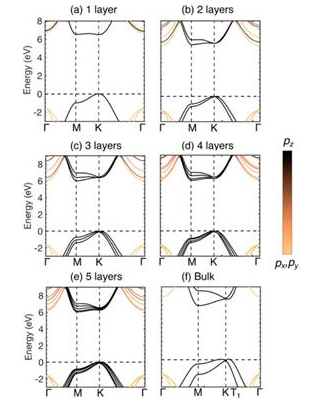
\includegraphics[width=.45\textwidth]{Figures/hBN-Layers}
  \caption{The variations in the bandgaps of hBN for each layer count \cite{jb1}}
  \label{fig:2}
\end{figure}
 
\subsection{Synthesizing hBN}

The synthesis of hBN is an ongoing challenge, in which its solution could provide a gateway for the commercialization of a variety of hBN sensors. Currently, one common method of synthesis is through chemical vapor deposition (CVD), a process in which a solid material is deposited on a substrate through chemical reactions involving a gaseous phase. This has been found to be the most consistent way to synthesize hBN, but large-scale production of hBN has not been achieved.

\subsubsection{Monolayer Synthesis}

Per Li et. Al, single-crystal hBN monolayers have been created, which is revolutionary for the future applications of hBN. To accomplish this synthesis, it is important to note the structure of the lattice of hBN. The structure of hBN suggests that a triangular lattice pattern is stronger than that of a hexagonal lattice, making for a more stable configuration on the metal substrates (Cu111 in this case) during synthesis \cite{jb2}. Typical CVD synthesis of hBN involves the introduction of ammonia borane thermally decomposing and being introduced into a heated chamber ($\approx1000[\si{\celsius}]$) with argon carrier gas \cite{jb2}. This then forms an hBN film of primarily triangular structures onto the Cu substrate. Interestingly, when a small amount of oxygen was diluted into the argon carrier gas, the hBN structures took the form of a hexagonal lattice \cite{jb3}. This is critical as these hexagonal structures can form a quality hBN monolayer, whereas the triangular lattices typically seen cannot. This is important to future applications of hBN due to the capability of these monolayer sheets to create reliable wafers (similar to a Si wafer) of hBN van der Waals heterostructures, whose implementations will be seen in high-reliability electronic devices \cite{jb1}.

\subsubsection{Multilayer Synthesis}

As discussed in the previous section, monolayer hBN is able to be synthesized utilizing CVD onto a transition metal thin film, but creating multilayer hBN has proven challenging. The rationale for the desire of multilayer over monolayer comes from the effects that multilayer hBN can produce, including improving optical properties of transition metal dichalcogenides, as well as for various DUV devices. Additionally, multilayer hBN films can reduce the influences of SiO$_2$ surfaces due to their thickness, while monolayers can not \cite{jb3}. This is a crucial fact when considering the field-effect transistors being developed utilizing multilayer hBN alongside graphene and SiO$_2$ (substrate), such that the hBN screens the impurities of the SiO$_2$ (dangling bonds, charge impurities) to improve the intrinsic carrier mobility \cite{jb2}.

To synthesize multilayer hBN, Fukamachi et. al, reports successful growth on Fe-Ni alloy foils utilizing CVD. These multilayer stacks were then used to create heterostacks with graphene to create functional FETs, outperforming the SiO$_2$-based ones. The process to accomplish this proves to be scalable, thus creating a gateway for the mass production of more efficient FET devices. The FETs created through this process had very high carrier mobilities (a maximum hole mobility of $10,219[\si{\centi\meter\squared\per\volt\per\second}]$, with an average of $5,477[\si{\centi\meter\squared\per\volt\per\second}]$) and electron mobility of $9,571[\si{\centi\meter\squared\per\volt\per\second}]$ (with an average of $5,551[\si{\centi\meter\squared\per\volt\per\second}]$) \cite{jb3}. This provides much hope for the future of 2D electronic devices, such that this observed high carrier mobility could reform the semiconductor industry in regard to 2D material implementation.

  \subsection{Applications}

  \subsubsection{DUV LEDs}

  These LEDs are used in a plethora of applications, including sterilization, water purification, photocatalysis, and curing processes \cite{jb2}. The current norm of these applications utilizes AlGaN semiconductors, but the issue is that these semiconductors emit light perpendicular to the surface of the plane. This makes for a weaker beam than if the light was emitted parallel to the plane, which is the case for an hBN DUV LED. This allows for a stronger beam, which in a process such as sterilization is crucial as it will be much more effective in neutralizing unwanted agents \cite{jb1}.

  \subsubsection{DUV PDs}

  Deep ultraviolet photodetectors, like DUV LEDs, are currently made with primarily AlGaN or GaN-based semiconductors, SiC semiconductors, amongst other similar 2D materials \cite{jb1}. The purpose of these photodetectors applies to a range of applications including flare detection systems, air purification devices, and advanced communication technologies. hBN has been developed into multiple different DUV-PDs, which have been obtained due to its bandgap lying within the DUV region. It has been found that the addition of another material (such as copper whilst creating a Schottky junction), as well as the addition of graphene for heterostructures, allows for a much more responsive PD than that of a single-hBN-based PD \cite{jb1}.

  \subsubsection{Perfect IR Absorbers/Emitters}

  hBN holds much promise in the realm of photonic devices operating in the infrared (IR) region \cite{jb2}, for specific applications such as radiative cooling, IR sensors, and biosensing. hBN is a viable suitor for such devices due to its inherent hyperbolic properties, enabling strong light confinement and efficient emission/absorption. By adjusting layer count and thickness, the thermal radiation and absorption properties can be tuned, such as creating a device with exact specifications for a variety of applications \cite{jb1}. The driving factor in utilizing hBN for these devices is its efficiency, as the current IR devices, although efficient, lack the tremendous efficiency seen by hBN within these applications. There is still much to be done in the form of research, but the future of IR appears to definitively have hBN involved.

\section{Silicene — Owen Chiu}

Similar to graphene, silicene is a 2D hexagonal structure, except with silicon atoms instead of carbon. Unlike graphene, silicene adopts a periodically buckled topology, where the atoms alternate being in the upper or lower positions (while still being a 1 atom thick layer).

This buckling behaviour is caused by differences in the sp hybridization of C and Si. For carbon, $sp^2$ is energetically favorable, while $sp^3$ hybridization is more favorable for silicon. This difference precludes many of the manufacturing techniques for graphene being applicable to silicene \cite{oc1}.

Similar to bulk silicon, silicene easily oxidizes when exposed to normal atmospheric conditions, which ruins its desired properties. Bulk silicon is normally put through a thermal oxidization process as part of the semiconductor manufacturing process, however this approach does not work for 2D materials. Proposed solutions to this problem include complete encapsulation (likely with polymers or metal oxides) and passivation. Depending on the elements introduced in the passivation process, new behaviours can be introduced to the silicene \cite{oc2}.

One of the intersting properties of silicene is its bandgap. Being a semi-metal, unmodified silicene does not have a bandgap, making it useless for semiconductor applications. Luckily, the bandgap of silicene can be modified using many different approaches. Topological changes, such as forming nanoribbons, can affect the bandgap, as can the substrate that the silicene is manufactured on. The introduction of other elements into or in between the silicene structure can also create a bandgap, including any materials introducted to prevent oxidization of the silicene. Finially, silicene's bandgap is vulnerable to modification by external electric fields \cite{oc2}.

Despite the challenges with silicene production, it has the possibility to provide breakthroughs in semiconductor development. The inherently smaller size of silicene compared to bulk silicon can provide immediate benefits in the miniturization of transistors, while the stacking of silicene layers provides opprotunities for the development of new types of transistors \cite{oc2,oc1}.

\section{Molybdenum Disulfite (MoS$_2$) — Oluwalaanu Adeboye}

Two-dimensional (2D) semiconducting materials, particularly MoS$_2$, have shown promise for electronic and optoelectronic applications due to their high mobility. However, achieving high-performance devices requires addressing several challenges, including improving 2D material quality, optimizing dielectrics, and reducing contact resistance. While significant progress has been made in optimizing fabrication processes and reducing defect density, further research is needed to address stability issues and enhance device performance for practical applications.

\begin{itemize}

  \item  TMDCs [DEFINE ACRONYMS ON FIRST USE] are layered compounds with MX$_2$ structure, where a covalently-bonded atomic plane of transition metal (M: groups IV to VII elements) is sandwiched between two atomic planes of chalcogen atoms (X: S, Se, and Te). These three-atom-thick monolayers are held together by weak van der Waals force, forming a layered structure as shown in crystal structure of MoS2 in figure 1(a) [WHAT IS THIS REFERRING TO?]. TMDCs have different electrical and optical properties depending on their chemical compositions, crystal structures, number of layers, and layer stacking sequence. 

\end{itemize}

\subsection{Uses of MoS$_2$}

\begin{itemize}

  \item 2D Tunneling Devices — ``Vertical tunneling devices based on vdW heterostructures show a steep transition slope of turn-on current at low power due to the sharpness of the band edges in atomically smooth hetero-interfaces. As shown in figure 7(a), the vertically-stacked 2D tunnel transistors were demonstrated by using atomically thin tunnel barriers of h-BN or MoS2 sandwiched between top and bottom graphene layers.''

  \item 2D Memories — ``2D memory devices, widely used for electronic non-volatile memories, have been realized by introducing atomically thin charge-trapping layers that act as floating gate in vertical vdW heterostructures. As shown in figure 8(a), Choi et al reported two different types of memory devices based on 2D vdW heterostructures. The first type had graphene as channel, h-BN as tunnel barrier, and MoS2 as charge-trapping layer. This device exhibited a large gate hysteresis window (~20 $\si{V}$) but a very low on/off ratio (~2), due to the zero bandgap and high mobility (4200 $\si{\centi\meter\squared\per\volt\per\second}$) of graphene. The second type of memory device had MoS$_2$ as channel and graphene as charge-trapping layer and showed high program/erase current ratio (~105), large memory window (18 $\si{\volt}$) and low operation voltage (50 $\si{\milli\volt}$), despite the low mobility (40 $\si{\centi\meter\squared\per\volt\per\second}$) of the MoS$_2$ channel. Those device parameters are competitive with those attained by organic transistor memory devices. Vu et al similarly developed two-terminal floating-gate memories with MoS2 channel, graphene floating gate and h-BN tunnel barrier.''

\end{itemize}

\section{2D Materials in Electronics — Daniela Salazar}

\subsection{Semiconductor Integration}

\begin{itemize}

  \item Chemical Vapor Deposition (CVD)

    \begin{itemize}

      \item Process were gas is in a reaction chamber, the gases then react and decompose in a heard surface which form a thin solid film 

      \item It is an essential for 2D material to synthesize thin layers and some of these steps include precursors, substrate preparation, and growth conditions 

      \item CVD is crucial in semiconductor manufacturing 

        \begin{itemize}

          \item Low Pressure CVD — this is used for highly uniformed films over large wafers 

          \item Metal Organic CVD

            \begin{itemize}

              \item This is common in the growth of III-V semiconductors used for electronic devices 

            \end{itemize}

        \end{itemize}

      \item The importance of using CVD for 2D Materials and Semiconductors 

        \begin{itemize}

          \item Control of the thickness precisely 

          \item It can be scaled for large-area growth 
            
          \item Less defect with higher crystal quality

          \item It is suitable for complex materials 

        \end{itemize}

      \item Adhesive Wafer Bonding 

        \begin{itemize}

          \item This is a proces that is used to bond two wafers with an adhesive layer and it is valuable to integrate delicate materials 

          \item Adhesive wafer bonding functions: 

            \begin{itemize}

              \item Begins by preparing the surface & ensuring there isn’t contamination 

              \item Then a polymer based adhesive is interested onto the wafers & then they are aligned and put in contact 

              \item The adhesive is then cured 

            \end{itemize}

          \item Importance in Semiconductors 

            \begin{itemize}

              \item Integrating materials onto silicon for photonic devices 

              \item Enable 3D integration in advanced chip designs 

              \item It also facilitates temperature sensitive materials bonding without the need for excessive heat exposure 

            \end{itemize}

        \end{itemize}

    \end{itemize}

  \item Van der Waals Forces 

    \begin{itemize}

      \item A lot of 2D materials (graphene, MoS2 \& h-BN) are composed of small layer that are held by these forces 

      \item The interactions are necessary for the structure 

      \item Importance in 2D Materials 

        \begin{itemize}

          \item Layered structure stability 

          \item Van der Waals Heterostructures 

          \item Clean interfaces 

        \end{itemize}

    \end{itemize}

  \item Transfer Techniques 

\end{itemize}

\subsection{Applications}

\begin{itemize}

  \item Enhance electronic devices 

    \begin{itemize}

      \item Ultra thin channels for transistors 

      \item Improves mobility \& conductivity 

      \item Flexible and transparent electronics 

    \end{itemize}

  \item Back end of line integration 

    \begin{itemize}

      \item Low-temperature processing 

      \item Atomic thinness for narrow spaces 

      \item Reduce capacitance 

    \end{itemize}

  \item Quantum computing 

    \begin{itemize}

      \item Topological insulators 

      \item Atomically shaped interfaces 

      \item Bandgaps that are tunable 

    \end{itemize}

  \item Buffer layer technique 

    \begin{itemize}

      \item Stress reduction

      \item Interface quality is enhanced

    \end{itemize}

\end{itemize}

\section{Flexible Electronics with 2D Materials — Thomas Czartoryski}

Flexible electronics refer to devices and circuits that are printed on stretchable and bendable substrates. This in turn allows for the integration of electronic components in applications where rigid devices and circuits are impractical such as biomedical sensors and wearable devices. The multifunctional properties of 2D materials make them promising candidates for flexible electronics in applications ranging from sensing to wireless communication. These properties range from good carrier mobility, flexibility, electrostatic control, extremely high optical constants, and the ability to scale down to one atomic layer \cite{tc1}. The materials that will be examined in this section for their usage in flexible electronics include graphene, black phosphorus (BP), and transition metal dichalcogenides (TMDs).

\subsection{Black Phosphorus}

Black Phosphorus (BP), is a popular 2D material used in flexible electronics. BP is an allotrope of phosphorus, and is phosphorus's most stable form, composed of layers held together by van der Waals forces. At a single layer it is called phosphorene and has a puckered honeycomb structure which results in direction-dependent electrical, optical, and mechanical properties \cite{tc2,tc3}. In addition, due to its puckered honeycomb structure, a monolayer of BP can sustain tensile strain up to 30\% and has a bandgap that is tunable in a range of $0.3[\si{eV}]$ in bulk and up to $2.0[\si{eV}]$ in a monolayer \cite{tc3}. One drawback of BP is that it oxides quickly which means that, unless it is encapsulated, it does not have long term stability. Part of the appeal of BP is its high speed and low energy consumption when compared to other 2D materials such as graphene and TMDs \cite{tc2}. The zero bandgap of graphene results in low-field effect modulation and a high `\textsc{OFF}' state current which makes digital or complementary meta-oxide-semiconductor (CMOS) logic implementations virtually impossible. TMDs, despite their large band gap and large `\textsc{ON/OFF}' current ratio, have a room temperature carrier mobility range of $10-100[\si{\centi\meter\squared\per\volt\per\second}]$, which is less than ideal for high-frequency applications \cite{tc4}. BP has a high room temperature carrier mobility ($\approx1000[\si{\centi\meter\squared\per\volt\per\second}]$). Wang et al. \cite{tc4} developed a top-gated transistor using BP which was found to have a cutoff frequency of up to $20[\si{\giga\hertz}]$, and a saturation velocity of $6\cdot10^6[\si{\centi\meter\per\second}]$. Additionally, the device, when tested under 1.5\% stretch, still performed well which makes it ideal for flexible electronics, and particularly for flexible radio frequency (RF) devices such as wearable sensors or communication devices.

\subsection{Graphene}

Graphene is used in flexible electronics due to its mechanical and electrical properties. Graphene has fracture strains of 25\%, good optical transmittance, high carrier mobility ($10,000[\si{\centi\meter\squared\per\volt\per\second}]$ at room temperature), and good piezoresistive sensitivity \cite{tc1}. Graphene has been used in a variety of flexible electronic applications including logic devices, energy-harvesting devices, sensors for e-skin applications, and biomedical devices. E-skin are electronic systems able to mimic the properties of human skin, such as flexibility, stretchability, biocompatibility, and able to detect changes in pressure, temperature, and humidity. The application of graphene in E-Skin is particularly groundbreaking because it incorporates all the use cases of graphene including, but not limited to, pressure and temperature sensors, nanogenerators, and flexible transistors \cite{tc1}. Graphene is used to develop tactile/pressure sensors due to its resistance to oxidation, high electrical conductivity ($106[\si{\siemen\per\meter}]$), and its ability to be both thin and flexible. Zhu et. al \cite{tc5} developed a tactile sensor with Graphene that was able to achieve response times of $0.2[\si{\milli\second}]$ and sensitivity to touch of up to $-5.53[\si{\per\kilo\pascal}]$. Graphene has been used in the development of liquid crystal displays (LCDs), organic light-emitted diodes (OLEDs), and touchscreens due to its optical, electrical, and mechanical properties. Graphene is highly transparent with 97.7\% of light transmission in a monolayer. Anagnostopoulos et al. \cite{tc6} investigated the mechanical behavior of a graphene-based flexible touch display. Two layers of graphene were embedded within a polyethylene terephthalate film via chemical vapor deposition. This screen, when bent or stretched, started to deform into separated patches or `islands', although this lowered electrical conductivity. The screen did not shatter like a traditional glass screen, and was able to withstand damage to the screen with up to 3\% uniaxial tension, which is an improvement on tempered glass screens which can only withstand 0.2-0.3\% uniaxial tensile strain before cracking \cite{tc6}. Graphene has also been used to develop flexible graphene field-effect transistors (GFETs). By depositiving graphene onto flexible substrates via chemical vapor deposition, GFETs can be created that have favorable mechanical and electrical properties. GFETs have been shown to withstand strain of up to 1.75\%, compared to traditional silicon field-effect transistors (FETs) which are brittle and can withstand less than a 0.1\% strain. GFETs have an extremely fast carrier transport, theoretically up to $200,000[\si{\centi\meter\squared\per\volt\per\second}]$, which make them ideal for communication devices (RF). A weakness of GFET is that it has no bandgap and a low `\textsc{ON/OFF}' ratio which makes them unsuitable for digital or CMOS logic \cite{tc7}.

\subsection{Transition Metal Dichalcogenides (TMDs)}

Another series of popular 2D materials used in flexible electronics are transition metal dichalcogenides (TMDs). TMDs are composed of a few atom polyhedral layers with transition metal atoms sandwiched between layers of chalcogen atoms. TMDs have been used in flexible FETs, flexible photodetectors, flexible sensors, and flexible memory devices \cite{tc1}. TMDs are particularly useful in high-performance flexible nanoscale FETs. The most common TMDs in the development of FETs are molybdenum disulfide (MoS$_2$) and tungsten diselenide (WSe$_2$). Unlike graphene, which lacks a band gap and has low resistivity, which  makes digital logic impossible, TMDs have band gaps similar to Silicon ($2[\si{eV}]$), and have led to mobilities of up to $470[\si{\centi\meter\squared\per\volt\per\second}]$ \cite{tc8}. Daus et. al \cite{tc8} utilized a new transfer process that resulted in the highest on-currents to date in $50[\si{\nano\meter}]$ channels. High performance MoS$_2$ transistors were developed on flexible substrates that enabled channels of $50[\si{\nano\meter}]$, which are the shortest to date in 2D material flexible electronics. Additionally, TMD FETs were able to withstand up to a 2\% strain which makes them a perfect candidate for flexible electronics \cite{tc8}. TMD nanosheets such as MoS$_2$ and MoSe$_2$ embedded in polymer matrices make for effective photodetectors due to their ability to absorb light across a wide spectrum. As a result, TMD can be particularly useful for foldable cameras and flexible optical sensors in applications such as robotics and wearables.  Velusamy et. al \cite{tc9} developed photodetectors by encapsulating TMD nanosheets in polymer matrices to prevent degradation. The MoSe$_2$ composite photodetectors achieved `\textsc{ON/OFF}' photo current ratios of $105$, which did not change even when bent at $200[\si{\meter}]$. In addition to this, by blending MoS$_2$, which detects visible light, and MoSe$_2$, which detects near-infrared light, the device could selectively detect and cover both visible and near-infrared wavelengths. The photodetector was still able to maintain consistent performance even when under mechanical strain, which highlights its ability to be used in flexible electronics. The TMD composite photodetectors were subjected to 1,000 bending cycles at a radius of $1[\si{\milli\meter}]$ and still worked without any deterioration in their performance \cite{tc9}.

\section{Conclusion \& Future Outlooks}

The future for hexagonal boron nitride is extensive, and there will undoubtedly be much to see with this material in the coming years. Once multilayer synthesis of hBN is commercialized, there will be great strides within the sanitation and medical industries, due to the advantages a multilayer hBN DUV LED has over the current ones, such as a stronger and more direct illumination. Furthermore, a multilayer hBN and graphene FET have already been created; thus, we can expect to see the commercialization of this device, which has been shown to improve the efficiency of the FET. Finally, in the RF realm in particular that of an effective RF capacitor. Due to its tremendously low-loss dielectric properties at high frequencies, making it a viable option for future implementations within the RF realm.

\section*{References}

\begin{center}
  \underline{Annotated Bibliography}
\end{center}

\subsection{Michael Brodskiy}

\subsubsection{Source \cite{mb4}}

This source provides in-depth insight into the properties and applications of graphene. This comprehensive paper discusses the fundamental aspects of graphene's electronic properties, including its unique band structure, and explores potential applications in electronic devices and materials science. The authors provide a detailed examination of experimental techniques for graphene synthesis and characterization, as well as future directions for research in graphene-based materials. This source serves as a foundational reference that helps to contextualize the transformative potential of graphene in modern electronics, and can possibly be dubbed one of the ``father sources'' of graphene's electrical applicability. By highlighting both theoretical and experimental perspectives, the authors create a comprehensive guide for researchers and industry professionals alike interested in graphene and its applications in electronic materials.

\subsubsection{Source \cite{mb5}}

This source discusses the graphene's emerging applicabiity due to its versatile functions and potential applications across various fields, including energy, medicine, and the defense industry. Notably, graphene's role in electromagnetic wave absorption and shielding has been a focal area of research. The review explores the structures and electromagnetic properties of graphene hybrids while discussing relaxation, charge transport, magnetic resonance, and eddy currents (an important topic when considering losses). It emphasizes the importance of magnetic-dielectric synergistic effects and centers on various graphene-based systems. The review focuses specifically on flexible graphene, graphene hybrids, and three-dimensional graphene architectures (however only 2D graphene was of interest for our purposes). As an individual who has personally worked on electromagnetic shielding and interference testing within the defense industry, this source was especially of interest to me.

\begin{thebibliography}{00}
\bibitem{intro} M. C. Lemme, D. Akinwande, C. Huyghebaert, and C. Stampfer, “2D materials for future heterogeneous electronics,” Nature Communications, vol. 13, no. 1, p. 1392, Mar. 2022, doi: https://doi.org/10.1038/s41467-022-29001-4.
\bibitem{mb3} Bolotin, K. I., Sikes, K. J., Jiang, Z., Fudenberg, G., Hone, J., Kim, P., & Stormer, H. L. (2008). Ultrahigh electron mobility in suspended graphene. Solid State Communications, 146(1-3), 351-355.
\bibitem{jb3} Fukamachi, S., Solís-Fernández, P., Kawahara, K. et al. Large-area synthesis and transfer of multilayer hexagonal boron nitride for enhanced graphene device arrays. Nat Electron 6, 126–136 (2023). https://doi.org/10.1038/s41928-022-00911-x
\bibitem{oc1} C. Grazianetti, E. Cinquanta, and A. Molle, “Two-dimensional silicon: the advent of silicene,” 2D Mater., vol. 3, no. 1, p. 012001, Jan. 2016, doi: 10.1088/2053-1583/3/1/012001.
\bibitem{mb1} Novoselov, K. S., Geim, A. K., Morozov, S. V., Jiang, D., Zhang, Y., Dubonos, S. V., ... & Firsov, A. A. (2004). Electric field effect in atomically thin carbon films. Science, 306(5696), 666-669.
\bibitem{mb2} Geim, A. K., & Novoselov, K. S. (2007). The rise of graphene. Nature materials, 6(3), 183-191.
\bibitem{mb4} Castro Neto, A. H., Guinea, F., Peres, N. M. R., Novoselov, K. S., & Geim, A. K. (2009). The electronic properties of graphene. Reviews of modern physics, 81(1), 109.
\bibitem{mb5} A. J. B. A. da Silva, C. R. S. de Lima, J. M. de Lima, C. T. M. G. dos Anjos, J. T. da Silva, and A. F. de Lima, "Graphene nanohybrids: excellent electromagnetic properties for the absorbing and shielding of electromagnetic waves," *J. Mater. Chem. C*, vol. 6, no. 46, pp. 12547-12559, 2018, doi: 10.1039/C7TC05869A.
\bibitem{mb6} Balandin, A. A., Ghosh, S., Bao, W., Calizo, I., Teweldebrhan, D., Miao, F., & Lau, C. N. (2008). Superior thermal conductivity of single-layer graphene. Nano letters, 8(3), 902-907.
\bibitem{mb7} Wang, X., Li, Q., & Zhang, Y. (2012). Graphene-based flexible electronics. Journal of materials chemistry, 22(13), 5965-5978.
\bibitem{mb8} Balandin, A. A. (2008). Thermal conductivity of graphene and graphene-based composites. Nano letters, 8(11), 3435-3437.
\bibitem{mb9} Li, X., Wang, X., Zhang, Y., & Bao, W. (2010). Graphene: A versatile material for flexible electronics. Advanced Materials, 22(35), 3877-3890.
\bibitem{jb1} Ogawa S, Fukushima S, Shimatani M. Hexagonal Boron Nitride for Photonic Device Applications: A Review. Materials (Basel). 2023 Feb 28;16(5):2005. doi: 10.3390/ma16052005. PMID: 36903116; PMCID: PMC10004243. 
\bibitem{jb2} Li, J., Samad, A., Yuan, Y. et al. Single-crystal hBN Monolayers from Aligned Hexagonal Islands. Nat Commun 15, 8589 (2024). https://doi.org/10.1038/s41467-024-52944-9
\bibitem{oc2} A. Molle, C. Grazianetti, L. Tao, D. Taneja, Md. H. Alam, and D. Akinwande, “Silicene, silicene derivatives, and their device applications,” Chem. Soc. Rev., vol. 47, no. 16, pp. 6370–6387, 2018, doi: 10.1039/C8CS00338F.
\bibitem{oc3} A. Kara et al., “A review on silicene — New candidate for electronics,” Surface Science Reports, vol. 67, no. 1, pp. 1–18, Jan. 2012, doi: 10.1016/j.surfrep.2011.10.001.
\bibitem{tc1} L. Gao, "Flexible device applications of 2D semiconductors," \textit{Small}, vol. 13, no. 25, p. 1603994, 2017, doi: 10.1002/smll.201603994.
\bibitem{tc2} R. K. Mishra, J. Sarkar, I. Chianella, S. Goel, and H. Y. Nezhad, "Black phosphorus: The rise of phosphorene in 2D materials applications," \textit{Next Materials}, vol. 4, p. 100217, 2024, doi: 10.1016/j.nxmate.2024.100217.
\bibitem{tc3} Q. Wei and X. Peng, "Superior mechanical flexibility of phosphorene and few-layer black phosphorus," \textit{Applied Physics Letters}, vol. 104, no. 25, p. 251915, Jun. 2014, doi: 10.1063/1.4885215.
\bibitem{tc4} H. Wang, X. Wang, F. Xia, L. Wang, H. Jiang, Q. Xia, M. L. Chin, M. Dubey, and S.-J. Han, "Black phosphorus radio-frequency transistors," \textit{Nano Letters}, vol. 14, no. 11, pp. 6424–6429, Nov. 2014, doi: 10.1021/nl5029717.
\bibitem{tc5} B. Zhu, Z. Niu, H. Wang, W. R. Leow, H. Wang, Y. Li, L. Zheng, J. Wei, F. Huo, and X. Chen, "Microstructured graphene arrays for highly sensitive flexible tactile sensors," \textit{Small}, vol. 10, no. 18, pp. 3625–3631, 2014, doi: 10.1002/smll.201401207.
\bibitem{tc6} G. Anagnostopoulos, P. N. Pappas, Z. Li, I. A. Kinloch, R. J. Young, K. S. Novoselov, C. Y. Lu, N. Pugno, J. Parthenios, C. Galiotis, and K. Papagelis, "Mechanical stability of flexible graphene-based displays," \textit{ACS Applied Materials \& Interfaces}, vol. 8, no. 34, pp. 22605–22614, Aug. 2016, doi: 10.1021/acsami.6b05227.
\bibitem{tc7} N. Petrone, I. Meric, J. Hone, and K. L. Shepard, "Graphene field-effect transistors with gigahertz-frequency power gain on flexible substrates," \textit{Nano Letters}, vol. 13, no. 1, pp. 121–125, Dec. 2012, doi: 10.1021/nl303666m.
\bibitem{tc8} A. Daus, S. Vaziri, V. Chen, C. Koroglu, R. Grady, C. Bailey, H. Lee, K. Brenner, K. Schauble, and E. Pop, "High-performance flexible nanoscale field-effect transistors based on transition metal dichalcogenides," \textit{arXiv preprint arXiv:2009.04056}, 2020, doi: 10.48550/arXiv.2009.04056.
\bibitem{tc9} D. Velusamy, R. Kim, S. Cha, \textit{et al.}, "Flexible transition metal dichalcogenide nanosheets for band-selective photodetection," \textit{Nature Communications}, vol. 6, p. 8063, 2015, doi: 10.1038/ncomms9063.
\end{thebibliography}

\end{document}
